\documentclass[11pt]{article}
\usepackage{forest}
\usepackage{float}

\usepackage[hmargin=1in,vmargin=1in]{geometry}
\usepackage{xcolor}
\usepackage{amsmath,amssymb,amsfonts,url,sectsty,framed,tcolorbox,framed}
\newcommand{\pf}{{\bf Proof: }}
\newtheorem{theorem}{Theorem}
\newtheorem{lemma}{Lemma}
\newtheorem{proposition}{Proposition}
\newtheorem{definition}{Definition}
\newtheorem{remark}{Remark}
\newcommand{\qed}{\hfill \rule{2mm}{2mm}}

\begin{document}
%%%%%%%%%%%%%%%%%%%%%%%%%%%%%%%%%%%%%%%%%%%%%%%%%%%%%%%%%%%%%%%%%%%%%
\noindent
\rule{\textwidth}{1pt}
\begin{center}
{\bf [CS304] Introduction to Cryptography and Network Security}
\end{center}
Course Instructor: Dr. Dibyendu Roy \hfill Winter 2023-2024\\
Scribed by: Sanidhya Kumar (202151138) \hfill Lecture (Week 4)
\\
\rule{\textwidth}{1pt}
%%%%%%%%%%%%%%%%%%%%%%%%%%%%%%%%%%%%%%%%%%%%%%%%%%%%%%%%%%%
%write here

\section{Groups}
We already saw what groups are. Let us quickly revise. A group $(G, \ast)$ consists of a set $G$ with a binary operation $\ast$ on $G$ satisfying the following three axioms:
\begin{enumerate}
    \item \textbf{Associativity}: $a \ast (b \ast c) = (a \ast b) \ast c$ for all $a, b, c \in G$.
    \item \textbf{Identity Element}: There is an element $1 \in G$, called the identity element, such that $a \ast 1 = 1 \ast a = a$ for all $a \in G$.
    \item \textbf{Inverse}: For each $a \in G$, there exists an element $a^{-1} \in G$, called the inverse of $a$, such that $a \ast a^{-1} = a^{-1} \ast a = 1$.
\end{enumerate}
\fbox{\parbox{\linewidth}{\textbf{Note}: A group $G$ is abelian (or commutative) if, furthermore, $a \ast b = b \ast a$ for all $a, b \in G$.}}


\subsection{Examples}
\begin{enumerate}
    \item $(G, \ast)$ where $G$ is the set of all invertible matrices.
    \item $(\mathbb{Z}, +)$
    \item $(\mathbb{Z}, \ast)$
    \item $(\mathbb{Z}, -)$
    \item $(\mathbb{Q}, \ast)$
    \item $(\mathbb{Q} - \{0\}, \ast)$
    \item $(\mathbb{Z}_n, +_n)$ \\\\
    Let's check if $(\mathbb{Z}_n, +_n)$ is a group or not where the set $\mathbb{Z}_n$ contains integers from $0$ to $n - 1$ (inclusive), and the operation $+_n$ is defined as $x +_n y = (x + y) \mod n$.
    \begin{itemize}
        \item Checking for associativity:
        \begin{align*}
            (x +_n y) +_n z &= (((x + y) \mod n) + z) \mod n \\
            &= (x + (y + z) \mod n) \mod n \\
            &= x +_n (y +_n z)
        \end{align*}
        Hence, $(\mathbb{Z}_n, +_n)$ is associative.
        
        \item Checking for identity:
        $0$ is the identity element as $x +_n 0 = x = 0 +_n x$.
        
        \item Checking for inverse:
        For any $x$ in $\mathbb{Z}_n$, the inverse of $x$ is $n - x$, since:
        \begin{align*}
            x +_n (n - x) &= (x + (n - x)) \mod n \\
            &= n \mod n \\
            &= 0
        \end{align*}
        Thus, every element in $\mathbb{Z}_n$ has an inverse.
    \end{itemize}
    Therefore, $(\mathbb{Z}_n, +_n)$ is a group, and it's also an abelian group.
    
    \item Let's check if $(\mathbb{Z}_n - \{0\}, \ast_n)$ is a group or not where the operation $\ast_n$ is defined as $(a, b) \ast_n (c, d) = (a \ast_1 c) \mod n \times (b \ast_2 d) \mod n$.
    \begin{itemize}
        \item This operation is associative on the given set.
        
        \item Identity Element: The identity element is $(1, 1)$.
        
        \item Inverse Element: The inverse of an element $(x, y)$, denoted as $(x^{-1}, y^{-1})$, exists only if $\gcd(x, n) = 1$ and $\gcd(y, n) = 1$. Hence, not every element in $(\mathbb{Z}_n - \{0\}) \times (\mathbb{Z}_n - \{0\})$ has an inverse under this operation.
        
        Hence, $(\mathbb{Z}_n - \{0\}, \ast_n)$ is a group if $\gcd(x, n) = 1$.
    \end{itemize}
\end{enumerate}

\subsection{Subgroups}
A non-empty subset $H$ of a group $(G, *)$ is a subgroup of $G$ if $H$ is itself a group with respect to the operation $*$ of $G$. If $H$ is a proper subset and a group with respect to $*$ of $G$ and $H \neq G$, then $H$ is called a proper subgroup of $(G, *)$. $H$ will have the following properties:
    \begin{enumerate}
            \item $H \subseteq G$
            \item $H$ is itself a group with $*$
    \end{enumerate}
    
Do note that $(G, *)$ is a group because $a \in G$, $a * a \in G$, $a * a * a \in G$,\\\\Here $*$ is just a notation for the operation which would be performed $a^i = a * a * a \dotsm a \in G$. A group $G$ is cyclic if there is an element $\alpha \in G$ such that for every $b \in G$, there is an integer $i$ with $b = \alpha^i$. This $\alpha$ is called the generator of $(G, *)$. Order of an element $a \in G$, $O(a)$, is the least positive integer $m$ such that $a^m = e$ (where $e$ is the identity element of $G$).

    \subsubsection{An Example} Given – $O(a) = 5$, $a^5 = e$. So, $S = \{e, a, a^2, a^3, a^4\}$ will be a subgroup of $G$ as:
    \begin{itemize}
        \item $S \subseteq G$ and
        \item $(S, *)$ is a group since it is associative, commutative, and has an inverse ($a^{-1} = a^4$ and so on).
        \item All elements in $S$ are generated by $a$ only. So, $a$ is a cyclic subgroup of $G$.
    \end{itemize}
\fbox{\parbox{\linewidth}{\textbf{Note:} Every subset of $G$ is not necessarily a subgroup.}}
\subsubsection{Cyclic Subgroups}

If $G$ is a group and $a \in G$, then the set of all powers of $a$ will form a cyclic subgroup generated by $a$ and denoted by $\langle a \rangle$. Let $G$ be a group and $a \in G$ be an element of finite order $t$, then $|\langle a \rangle|$ denotes the size of the subgroup generated by $a$ and equals $t$.

\subsubsection{Lagrange’s Subgroups}
If $G$ is a finite group and $H$ is a subgroup of $G$, then $|H|$ divides $|G|$. Since the order of the element generating the subgroup is equal to the cardinality of the subgroup, therefore, the order of the element also divides $|G|$.\\\\
Let $a \in G$ and $O(a)$ be the order of element $a$. Therefore,
\[ S = \{a^0, a^1, a^2, \ldots, a^{O(a) - 1}\} = \langle a \rangle \]
$(S, *)$ is a subgroup of $(G, *)$. \\\\
From Lagrange’s Theorem,
\[ |H| \text{ divides } |G| \Rightarrow O(a) \text{ divides } |G| \]

\subsection{Important Result}
If the order of $a \in G$ is $t$, then the order of $a^k$ is $t/\text{gcd}(t,k)$.

\[ \langle a \rangle = \{e, a, a^2, \ldots, a^{O(a)-1}\} \]

\[\langle at \rangle = \{e, ar, a^2t, \ldots, (at)^{O(at)-1}\}\]

\[B = at\]

\[\langle at \rangle = \langle b \rangle = \{e, b, b^2, \ldots, b^{O(b)-1}\}\]\\\\
If gcd(t, O(a)) = 1, then O(at) = O(a)


\section{Ring}
A ring $(R, +_R, \times_R)$ consists of one set $R$ with two binary operations arbitrarily denoted by $+_R$ (addition) and $\times_R$ (multiplication) on $R$ satisfying the following properties:
\begin{enumerate}
    \item $(R, +_R)$ is an abelian group with the identity element $0_R$.
    \item The operation $\times_R$ is associative, that is,
    \[ a \times_R (b \times_R c) = (a \times_R b) \times_R c \text{ for all } a, b, c \in R \]
    \item There is a multiplicative identity denoted by $1_R$ with $1_R \neq 0_R$ such that $1_R \times_R a = a \times_R 1_R = a$ for all $a \in R$.
    \item The operation $\times_R$ is distributive over $+_R$, that is,
    \[ (b +_R c) \times_R a = (b \times_R a) +_R (c \times_R a) \]
    \[ a \times_R (b +_R c) = (a \times_R b) +_R (a \times_R c) \]
\end{enumerate}

\fbox{\parbox{\linewidth}{\textbf{Note:} We do not worry about the inverse of $\times_R$.}}

\subsection{Examples}
\begin{enumerate}
    \item $(\mathbb{Z}, +, \cdot)$:
    \begin{itemize}
        \item $(\mathbb{Z},+)$: abelian group
        \begin{enumerate}
            \item Associativity: $a+(b+c) = (a+b)+c$
            \item Identity Element: $a+0=a=0+a$ (0 is the identity element)
            \item Inverse: $a+(-a)=0=(-a)+a$
            \item Abelian Property: $a+b = b+a$ for all $a,b \in \mathbb{Z}$
        \end{enumerate}
        \item $(\mathbb{Z},\cdot)$: 
        \item Distributive property: $a\cdot 1=1\cdot a=a$, where $1$ is the identity element.
        \item Distributive property: $a\cdot (b+c)=(a\cdot b)+(a\cdot c)$
        \item Distributive property: $(b+c)\cdot a=(b\cdot a)+(c\cdot a)$
    \end{itemize}
    
    \item $(\mathbb{R}, +_R, \times_R)$: $a \times_R b = b \times_R a$ for all $a,b \in \mathbb{R}$, hence it is a commutative ring.
    
    
    \item $(\mathbb{Z}, +, \cdot)$: Commutative ring.
\end{enumerate}

\subsection{Units}

An element $a$ of a ring $R$ is called a unit or an invertible element if there exists an element $b \in R$ such that $a \times_R b = 1_R$. (1 is the unit element in $(\mathbb{Z},+,\cdot)$). The set of units in a ring $R$ forms a group under the multiplication operation. This is known as the group of units of $R$. (Since, the inverse was missing and we added that as well).

\section{Field}
A field is a non-empty set $F$ together with two binary operations, addition $(+)$ and multiplication $(\cdot)$, for which the following properties are satisfied:
\begin{enumerate}
    \item $(F, +)$ is an abelian group.
    \item If $0_F$ denotes the additive identity element of $(F, +)$, then $(F - \{0_F\}, \cdot)$ is an abelian group.
    \item For all $a, b, c \in F$, we have $a \cdot (b + c) = (a \cdot b) + (a \cdot c)$.
\end{enumerate}

\subsection{Examples}
\begin{enumerate}
    \item $(\mathbb{Z}, +, \cdot)$: 
    \begin{itemize}
        \item $(\mathbb{Z}, +)$ is an abelian group with identity element $0$. 
        \item But for the set $\mathbb{Z} - \{0\}$, multiplicative inverse does not exist. Hence, $(\mathbb{Z} - \{0\}, \cdot)$ is not an abelian group. 
        \item Hence, $(\mathbb{Z}, +, \cdot)$ is not a field.
    \end{itemize}
    
    \item $(\mathbb{Q}, +, \cdot)$:
    \begin{itemize}
        \item $(\mathbb{Z}, +)$ is an abelian group with identity element $0$.
        \item For the set $\mathbb{Q} - \{0\}$, multiplicative inverse exists for every rational number.
        \item Multiplication is distributive over addition on rational numbers. Hence, $(\mathbb{Q}, +, \cdot)$ is a field.
    \end{itemize}
    
    \item $(\mathbb{F}_p, +_p, \cdot_p)$, where $\mathbb{F}_p = \{0,1,2,\ldots,p-1\}$ and $p$ is any prime number:
    \begin{itemize}
        \item $+_p$: $(x+y) \mod p$ - Trivially, this is an abelian group.
        \item $\cdot_p$: $(x \cdot y) \mod p$ - Remove $0$ from $\mathbb{F}_p$ then $\text{gcd}(x,p) = 1$ since $p$ is prime. Also, it is trivial that $\cdot_p$ is distributive over $+_p$.
        \item Hence $(\mathbb{F}_p, +_p, \cdot_p)$ is a field.
    \end{itemize}
\end{enumerate}

\subsection{Field Extension}
Suppose $K_2$ is a field with addition $(+)$ and multiplication $(\cdot)$. Suppose $K_1 \subseteq K_2$ is closed under both these operations such that $K_1$ itself is a field with the restriction of $+$ and $\cdot$ to the set $K_1$. Then $K_1$ is called a subfield of $K_2$ and $K_2$ is called a field extension of $K_1$.

\section{Polynomial Ring}
Let $(F, +, \ast)$ be a field. The set of polynomials of any degree $F[x]$ is defined as:
\[ F[x] = \{ a_0 + a_1 \cdot x + a_2 \cdot x^2 + \ldots | a_i \in F \} \]
The polynomial ring, denoted as $F[x]$, consists of all polynomials in the variable $x$ whose coefficients are elements of the field $F$. This ring is formed by combining the set of polynomials with the field's binary operations, thereby establishing a structure where polynomial addition and multiplication satisfy the ring properties.
\[ (F[x], +, \ast) \rightarrow \text{Polynomial Ring} \]\\
Let $P_1(x) \in F[x] = a_0 + a_1 \cdot x + \ldots + a_n \cdot x^n$ \\\\
$P_2(x) \in F[x] = b_0 + b_1 \cdot x + \ldots + b_n \cdot x^n$\\

If we want to add the two polynomials:
\[ P_1(x) + P_2(x) = (a_0 + a_1 \cdot x + \ldots + a_n \cdot x^n) + (b_0 + b_1 \cdot x + \ldots + b_n \cdot x^n) \]
\[ P_1(x) + P_2(x) = (a_0 + b_0) + (a_1 + b_1) \cdot x + \ldots + (a_n + b_n) \cdot x^n \]

Multiplication operation of the two polynomials:
\[ P_1(x) \ast P_2(x) = (a_0 + a_1 \cdot x + \ldots + a_n \cdot x^n) \ast (b_0 + b_1 \cdot x + \ldots + b_n \cdot x^n) \]
\[ P_1(x) \ast P_2(x) = (a_0 \ast b_0) + (a_0 \ast b_1 + b_0 \ast a_1) \cdot x + \ldots + (a_n \ast b_n) \cdot x^n \]

Additive inverse of $P(x)$:
\[ P(x) = a_0 + a_1 \cdot x + \ldots + a_n \cdot x^n \]
\[ P(-x) = -a_0 + (-a_1) \cdot x + \ldots + (-a_n) \cdot x^n \]
Clearly, $P(-x)$ is the additive inverse of $P(x)$. Here, the negative sign does not mean the standard negation.\\\\
A polynomial ring is formally defined as the set of all polynomials $F[x]$ along with the operations of addition $(+)$ and multiplication $(*),$ and it is referred to as a ring if it satisfies the following conditions:
\begin{enumerate}
    \item $(F[x], +)$ is an abelian group.
    \item $*$ is associative over $F[x]$.
    \item An identity element over multiplication exists.
    \item $*$ is distributive over $+$.
\end{enumerate}

\subsection{Example} Consider the set $F = \{0, 1\}$ and the field $(F, +_2, \ast_2)$. Therefore, the polynomial set $F_2[x]$ is:
\[ F_2[x] = \{a_0 + a_1 \cdot x + \ldots | a_i \in F\} \]
Let us take two example polynomials:
\[ p(x) = x + 1 \]
\[ q(x) = x^2 + x + 1 \]
\[ p(x) +_2 q(x) = (x + 1) +_2 (x^2 + x + 1) = x^2 + (1 +_2 1) \cdot x + (1 +_2 1) = x^2 \]
\[ p(x) \ast_2 q(x) = (x + 1) \ast_2 (x^2 + x + 1) \]
\[ p(x) \ast_2 q(x) = (x^3 + x^2 + x) + (x^2 + x + 1) = x^3 + (1 +_2 1) \cdot x^2 + (1 +_2 1) \cdot x + 1 \]
\[ p(x) \ast_2 q(x) = x^3 + 1 \]\\
Here, to get the coefficient of $x^i$, we will perform addition (of terms forming power $i$) or multiplication (of terms forming power $i$) modulo $2$ operation.

\section{Irreducible Polynomials}
A polynomial $P(x) \in F[x]$ of degree $n \geq 1$ is called irreducible if it cannot be written in the form of $P_1(x) \ast P_2(x)$ with $P_1(x), P_2(x) \in F[x]$ and the degree of $P_1(x), P_2(x)$ must be greater than or equal to $1$.

\subsection{Important Property}
$x^2+1$ belongs to $F_2[x]$.
\[ (x + 1) \ast (x + 1) = x^2 + (1 + 1) \ast x + 1 = x^2 + 1. \]
Therefore, $x^2 + 1 = (x + 1) \ast (x + 1)$ in $F_2[x]$. Hence, $x^2 + 1$ is reducible in $F_2[x]$. Now, consider a set denoted by $I$, containing polynomials defined as:
\[ I = \langle P(x) \rangle = \{ q(x) \ast P(x) | q(x) \in F[x] \} \]
Also, consider the set denoted by $F[x]/\langle P(x) \rangle$, where each element is formed by dividing an element from $F[x]$ by $P(x)$.\\\\
For any $q(x) \in F[x]$, there exist polynomials $d(x)$ and $r(x)$ such that:
\[ q(x) = d(x) \ast P(x) + r(x) \]
where $r(x) \in F[x]/\langle P(x) \rangle$.\\\\      
Also, if $P(x)$ is an irreducible polynomial, then $(F[x]/\langle P(x) \rangle, +, \ast)$ forms a field. In this context, addition and multiplication operations are performed modulo $P(x)$. Notably, the degree of $r(x)$ is always less than the degree of $P(x)$.

\subsection{Examples}
\begin{enumerate}
    \item $x^2+1$ in $\mathbb{R}[x]$:
    \begin{itemize}
        \item It is not possible to factor $x^2 + 1$ in $\mathbb{R}[x]$, where $\mathbb{R}$ is the set of real numbers.
        \item Let $P(x)=q_1(x) \cdot q_2(x)$.
        \item $\text{Deg}(q_1) \geq 1$
        \item $\text{Deg}(q_2) \geq 1$
        \item $x^2+1=0$
        \item $x^2=-1$
        \item $x=\pm i$
        \item $(x+\alpha)$ and $(x-\alpha)$
        \item It is not a reducible polynomial because to reduce, it would result in $(x+i)$ and $(x-i)$ which are complex numbers, but it is in $\mathbb{R}$ (Real numbers). So, it is irreducible.
    \end{itemize}
    
    \item $x^2 + x + 1$ in $\mathbb{F}_2[x]$, where $\mathbb{F}_2 = \{0, 1\}$:
    \begin{itemize}
        \item The polynomial $P(x) = x^2 + x + 1$ is irreducible.
        \item We will put $x = 0$ and $x = 1$:
        \item $P(0) = 1$
        \item $P(1) = 1$
        \item So, $(x + 0)$ and $(x + 1)$ are not factors of $P(x)$. There are no degree $1$ factors of this $P(x)$. Hence, it is irreducible.
    \end{itemize}
\end{enumerate}
Consider the set $\mathbb{F}_2[x]/\langle x^2 + x + 1 \rangle$: For any polynomial $q(x)$, we can express it as:
\[ q(x) = d(x) \cdot P(x) + r(x) \]
where $\text{deg}(d(x)) < 2$ and $\text{deg}(r(x)) < 2$. The possible remainders $r(x)$ can be $\{0, 1, x, x + 1\}$. If $P(x)$ is an $n$-degree polynomial under modulo $2$, then there will be $2^{2n}$ polynomials in $r(x)$, meaning $\mathbb{F}_2[x]/\langle x^2 + x + 1 \rangle$ will have $2^2 = 4^2 = 16$ polynomials.

\section{Primitive Polynomials}
Consider the set $\mathbb{F}_2[x]/\langle x^2+x+1 \rangle$. We've established that if $P(x)$ is irreducible, then $(\mathbb{F}_2[x]/\langle x \rangle, +, \ast)$ forms a field. Now, suppose $\alpha$ is a root of $x^2 + x + 1 = 0$, i.e., $\alpha^2 + \alpha + 1 = 0$. This implies $\alpha^2 = -\alpha - 1 = \alpha + 1$. If $\alpha$ can generate all possible polynomials in $\mathbb{F}_2[x]/\langle x^2 + x + 1 \rangle$, then $x^2 + x + 1$ is termed a primitive polynomial.\\\\
Let's demonstrate this:
\[ \langle \alpha \rangle = \{0, 1 = \alpha^0, \alpha, \alpha + 1 = \alpha^2\} \]
The order of $\alpha$, denoted as $O(\alpha)$, is $2$. Hence, $x^2 + x + 1$ is a primitive polynomial.

\subsection{Example}
Consider $\mathbb{F}_2[x]/\langle x^3+x+1 \rangle$. The maximum number of polynomials that can be generated: $\{0, 1, x, x+1, x^2, x^2 + 1, x^2 + x, x^2 + x + 1\}$.\\\\
Let's check if the root of $x^3 + x + 1 = 0$ is a generator:
\[ \alpha^3 + \alpha + 1 = 0 \Rightarrow \alpha^3 = \alpha + 1 \]
\[ \langle \alpha \rangle = \{0, 1 = \alpha^0, \alpha, \alpha^2, \alpha + 1 = \alpha^3, \alpha^2 + \alpha = \alpha^4, \alpha^2 + \alpha + 1 = \alpha^5, \alpha^2 + 1 = \alpha^6\} \]
Since we can generate all the polynomials, $x^3 + x + 1$ is a primitive polynomial.\\\\
Note that there may exist a polynomial that is not primitive but still forms a field. That implies we can find a multiplicative inverse. Consider the polynomial $\alpha x$. Instead of $1/\alpha x$, we have the polynomial $\alpha^2 + 1/x^2 + 1$, which results in $1$ on multiplication.
\[ x \cdot (x^2 + 1) = x^3 + x = x + 1 + x = 1 \]
Similarly, for $x^2$, the multiplicative inverse is $x^2 + x + 1$.
\[ x^2 \cdot (x^2 + x + 1) = x^4 + x^3 + x^2 = x \cdot (x + 1) + (x + 1) + x^2 \]
\[ x^2 \cdot (x^2 + x + 1) = x^2 + x + x + 1 + x^2 = 1 \]

\section{AES (Advanced Encryption Standard)}
After DES was found to be vulnerable once it was released to the public, a new competition was held named AES to find a better cipher. In the competition, Rindel was the winning cipher and hence according to the rules of the competition, it was renamed to AES. AES is a NIST Standardized iterated block cipher and a substitution permutation network (SPN) as well.\\\\
Let us see the variations of AES:
\begin{enumerate}
    \item \textbf{AES-128}:
    \begin{itemize}
        \item Block size – 128 bit
        \item Number of rounds – 10
        \item Secret Key size – 128
    \end{itemize}
    
    \item \textbf{AES-192}:
    \begin{itemize}
        \item Block size – 128 bit
        \item Number of rounds – 12
        \item Secret Key size – 192
    \end{itemize}
    
    \item \textbf{AES-256}:
    \begin{itemize}
        \item Block size – 128 bit
        \item Number of rounds – 14
        \item Secret Key size – 256
    \end{itemize}
\end{enumerate}
\textbf{Note:} In all these three, only the number of rounds and the secret key size change!

\subsection{Structure of AES}


\begin{center}
    \tikzset{every picture/.style={line width=0.75pt}}
    
    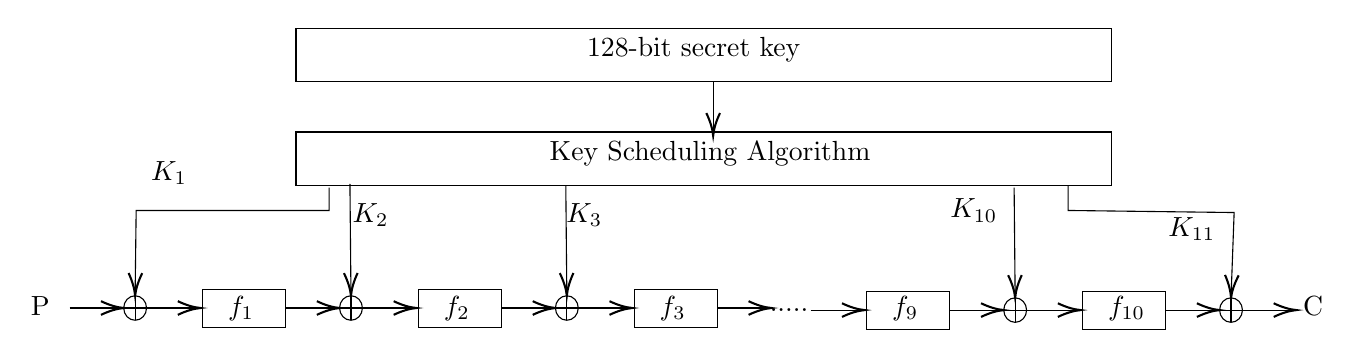
\begin{tikzpicture}[x=0.75pt,y=0.75pt,yscale=-1,xscale=1]
        \draw   (146,38) -- (539,38) -- (539,63.8) -- (146,63.8) -- cycle ;
        \draw    (347,63.8) -- (347,87.8) ;
        \draw [shift={(347,89.8)}, rotate = 270] [color={rgb, 255:red, 0; green, 0; blue, 0 }  ][line width=0.75]    (10.93,-3.29) .. controls (6.95,-1.4) and (3.31,-0.3) .. (0,0) .. controls (3.31,0.3) and (6.95,1.4) .. (10.93,3.29)   ; 
        \draw   (146,88) -- (539,88) -- (539,113.8) -- (146,113.8) -- cycle ;
        \draw    (37,172.8) -- (61,172.8) ;
        \draw [shift={(63,172.8)}, rotate = 180] [color={rgb, 255:red, 0; green, 0; blue, 0 }  ][line width=0.75]    (10.93,-3.29) .. controls (6.95,-1.4) and (3.31,-0.3) .. (0,0) .. controls (3.31,0.3) and (6.95,1.4) .. (10.93,3.29)   ;
        \draw   (63,172.8) .. controls (63,169.54) and (65.46,166.9) .. (68.5,166.9) .. controls (71.54,166.9) and (74,169.54) .. (74,172.8) .. controls (74,176.06) and (71.54,178.7) .. (68.5,178.7) .. controls (65.46,178.7) and (63,176.06) .. (63,172.8) -- cycle ; \draw   (63,172.8) -- (74,172.8) ; \draw   (68.5,166.9) -- (68.5,178.7) ;
        \draw    (74,172.8) -- (98,172.8) ;
        \draw [shift={(100,172.8)}, rotate = 180] [color={rgb, 255:red, 0; green, 0; blue, 0 }  ][line width=0.75]    (10.93,-3.29) .. controls (6.95,-1.4) and (3.31,-0.3) .. (0,0) .. controls (3.31,0.3) and (6.95,1.4) .. (10.93,3.29)   ;
        \draw   (101,163.8) -- (141,163.8) -- (141,182) -- (101,182) -- cycle ;
        \draw    (141,172.8) -- (165,172.8) ;
        \draw [shift={(167,172.8)}, rotate = 180] [color={rgb, 255:red, 0; green, 0; blue, 0 }  ][line width=0.75]    (10.93,-3.29) .. controls (6.95,-1.4) and (3.31,-0.3) .. (0,0) .. controls (3.31,0.3) and (6.95,1.4) .. (10.93,3.29)   ;
        \draw   (167,172.8) .. controls (167,169.54) and (169.46,166.9) .. (172.5,166.9) .. controls (175.54,166.9) and (178,169.54) .. (178,172.8) .. controls (178,176.06) and (175.54,178.7) .. (172.5,178.7) .. controls (169.46,178.7) and (167,176.06) .. (167,172.8) -- cycle ; \draw   (167,172.8) -- (178,172.8) ; \draw   (172.5,166.9) -- (172.5,178.7) ;
        \draw    (178,172.8) -- (202,172.8) ;
        \draw [shift={(204,172.8)}, rotate = 180] [color={rgb, 255:red, 0; green, 0; blue, 0 }  ][line width=0.75]    (10.93,-3.29) .. controls (6.95,-1.4) and (3.31,-0.3) .. (0,0) .. controls (3.31,0.3) and (6.95,1.4) .. (10.93,3.29)   ; 
        \draw   (205,163.8) -- (245,163.8) -- (245,182) -- (205,182) -- cycle ; 
        \draw    (245,172.8) -- (269,172.8) ;
        \draw [shift={(271,172.8)}, rotate = 180] [color={rgb, 255:red, 0; green, 0; blue, 0 }  ][line width=0.75]    (10.93,-3.29) .. controls (6.95,-1.4) and (3.31,-0.3) .. (0,0) .. controls (3.31,0.3) and (6.95,1.4) .. (10.93,3.29)   ; 
        \draw   (271,172.8) .. controls (271,169.54) and (273.46,166.9) .. (276.5,166.9) .. controls (279.54,166.9) and (282,169.54) .. (282,172.8) .. controls (282,176.06) and (279.54,178.7) .. (276.5,178.7) .. controls (273.46,178.7) and (271,176.06) .. (271,172.8) -- cycle ; \draw   (271,172.8) -- (282,172.8) ; \draw   (276.5,166.9) -- (276.5,178.7) ;
        \draw    (282,172.8) -- (306,172.8) ;
        \draw [shift={(308,172.8)}, rotate = 180] [color={rgb, 255:red, 0; green, 0; blue, 0 }  ][line width=0.75]    (10.93,-3.29) .. controls (6.95,-1.4) and (3.31,-0.3) .. (0,0) .. controls (3.31,0.3) and (6.95,1.4) .. (10.93,3.29)   ;
        \draw   (309,163.8) -- (349,163.8) -- (349,182) -- (309,182) -- cycle ;
        \draw    (349,172.8) -- (373,172.8) ;
        \draw [shift={(375,172.8)}, rotate = 180] [color={rgb, 255:red, 0; green, 0; blue, 0 }  ][line width=0.75]    (10.93,-3.29) .. controls (6.95,-1.4) and (3.31,-0.3) .. (0,0) .. controls (3.31,0.3) and (6.95,1.4) .. (10.93,3.29)   ;
        \draw    (394,173.8) -- (418,173.8) ;
        \draw [shift={(420,173.8)}, rotate = 180] [color={rgb, 255:red, 0; green, 0; blue, 0 }  ][line width=0.75]    (10.93,-3.29) .. controls (6.95,-1.4) and (3.31,-0.3) .. (0,0) .. controls (3.31,0.3) and (6.95,1.4) .. (10.93,3.29)   ;
        \draw   (421,164.8) -- (461,164.8) -- (461,183) -- (421,183) -- cycle ;
        \draw    (461,173.8) -- (485,173.8) ;
        \draw [shift={(487,173.8)}, rotate = 180] [color={rgb, 255:red, 0; green, 0; blue, 0 }  ][line width=0.75]    (10.93,-3.29) .. controls (6.95,-1.4) and (3.31,-0.3) .. (0,0) .. controls (3.31,0.3) and (6.95,1.4) .. (10.93,3.29)   ;
        \draw   (487,173.8) .. controls (487,170.54) and (489.46,167.9) .. (492.5,167.9) .. controls (495.54,167.9) and (498,170.54) .. (498,173.8) .. controls (498,177.06) and (495.54,179.7) .. (492.5,179.7) .. controls (489.46,179.7) and (487,177.06) .. (487,173.8) -- cycle ; \draw   (487,173.8) -- (498,173.8) ; \draw   (492.5,167.9) -- (492.5,179.7) ;
        \draw    (498,173.8) -- (522,173.8) ;
        \draw [shift={(524,173.8)}, rotate = 180] [color={rgb, 255:red, 0; green, 0; blue, 0 }  ][line width=0.75]    (10.93,-3.29) .. controls (6.95,-1.4) and (3.31,-0.3) .. (0,0) .. controls (3.31,0.3) and (6.95,1.4) .. (10.93,3.29)   ;
        \draw   (525,164.8) -- (565,164.8) -- (565,183) -- (525,183) -- cycle ;
        \draw    (565,173.8) -- (589,173.8) ;
        \draw [shift={(591,173.8)}, rotate = 180] [color={rgb, 255:red, 0; green, 0; blue, 0 }  ][line width=0.75]    (10.93,-3.29) .. controls (6.95,-1.4) and (3.31,-0.3) .. (0,0) .. controls (3.31,0.3) and (6.95,1.4) .. (10.93,3.29)   ;
        \draw   (591,173.8) .. controls (591,170.54) and (593.46,167.9) .. (596.5,167.9) .. controls (599.54,167.9) and (602,170.54) .. (602,173.8) .. controls (602,177.06) and (599.54,179.7) .. (596.5,179.7) .. controls (593.46,179.7) and (591,177.06) .. (591,173.8) -- cycle ; \draw   (591,173.8) -- (602,173.8) ; \draw   (596.5,167.9) -- (596.5,179.7) ; 
        \draw    (602,173.8) -- (626,173.8) ;
        \draw [shift={(628,173.8)}, rotate = 180] [color={rgb, 255:red, 0; green, 0; blue, 0 }  ][line width=0.75]    (10.93,-3.29) .. controls (6.95,-1.4) and (3.31,-0.3) .. (0,0) .. controls (3.31,0.3) and (6.95,1.4) .. (10.93,3.29)   ;
        \draw    (162,114.8) -- (162,125.8) -- (69,125.8) -- (68.52,164.9) ;
        \draw [shift={(68.5,166.9)}, rotate = 270.7] [color={rgb, 255:red, 0; green, 0; blue, 0 }  ][line width=0.75]    (10.93,-3.29) .. controls (6.95,-1.4) and (3.31,-0.3) .. (0,0) .. controls (3.31,0.3) and (6.95,1.4) .. (10.93,3.29)   ;
        \draw    (172,113) -- (172.48,164.9) ;
        \draw [shift={(172.5,166.9)}, rotate = 269.47] [color={rgb, 255:red, 0; green, 0; blue, 0 }  ][line width=0.75]    (10.93,-3.29) .. controls (6.95,-1.4) and (3.31,-0.3) .. (0,0) .. controls (3.31,0.3) and (6.95,1.4) .. (10.93,3.29)   ;
        \draw    (276,113.8) -- (276.48,164.9) ;
        \draw [shift={(276.5,166.9)}, rotate = 269.46] [color={rgb, 255:red, 0; green, 0; blue, 0 }  ][line width=0.75]    (10.93,-3.29) .. controls (6.95,-1.4) and (3.31,-0.3) .. (0,0) .. controls (3.31,0.3) and (6.95,1.4) .. (10.93,3.29)   ;
        \draw    (492,114.8) -- (492.48,165.9) ;
        \draw [shift={(492.5,167.9)}, rotate = 269.46] [color={rgb, 255:red, 0; green, 0; blue, 0 }  ][line width=0.75]    (10.93,-3.29) .. controls (6.95,-1.4) and (3.31,-0.3) .. (0,0) .. controls (3.31,0.3) and (6.95,1.4) .. (10.93,3.29)   ;
        \draw    (518,113.8) -- (518,125.8) -- (598,126.8) -- (596.57,165.9) ;
        \draw [shift={(596.5,167.9)}, rotate = 272.09] [color={rgb, 255:red, 0; green, 0; blue, 0 }  ][line width=0.75]    (10.93,-3.29) .. controls (6.95,-1.4) and (3.31,-0.3) .. (0,0) .. controls (3.31,0.3) and (6.95,1.4) .. (10.93,3.29)   ;
        
        \draw (285,41) node [anchor=north west][inner sep=0.75pt]   [align=left] {128-bit secret key};
        \draw (267,91) node [anchor=north west][inner sep=0.75pt]   [align=left] {Key Scheduling Algorithm};
        \draw (17,166) node [anchor=north west][inner sep=0.75pt]   [align=left] {P};
        \draw (112,166) node [anchor=north west][inner sep=0.75pt]   [align=left] {$f_1$};
        \draw (216,166) node [anchor=north west][inner sep=0.75pt]   [align=left] {$f_2$};
        \draw (320,166) node [anchor=north west][inner sep=0.75pt]   [align=left] {$f_3$};
        \draw (373,172) node [anchor=north west][inner sep=0.75pt]   [align=left] {.....};
        \draw (432,166) node [anchor=north west][inner sep=0.75pt]   [align=left] {$f_9$};
        \draw (536,166) node [anchor=north west][inner sep=0.75pt]   [align=left] {$f_{10}$};
        \draw (630,166) node [anchor=north west][inner sep=0.75pt]   [align=left] {C};
        \draw (75,101) node [anchor=north west][inner sep=0.75pt]   [align=left] {$K_1$};
        \draw (172,121) node [anchor=north west][inner sep=0.75pt]   [align=left] {$K_2$};
        \draw (275,121) node [anchor=north west][inner sep=0.75pt]   [align=left] {$K_3$};
        \draw (460,119) node [anchor=north west][inner sep=0.75pt]   [align=left] {$K_{10}$};
        \draw (565,128) node [anchor=north west][inner sep=0.75pt]   [align=left] {$K_{11}$};
    \end{tikzpicture}
\end{center}
Important Observations -
\begin{itemize}
    \item 10 Rounds
    \item 11 Keys Generated
    \item Ciphertext also of 128 bits
\end{itemize}




%%%%%%%%%%%%%%%%%%%%%%%%%%%%%%%%%%%%%%%%%%%%
%END
 
\end{document}